% !TEX encoding = UTF-8 Unicode

\documentclass{beamer}
\usepackage{beamerthemeshadow}
\usepackage{graphicx}
\usepackage{color}
\usepackage[utf8]{inputenc}
\usepackage{hyperref}
\usepackage[flushleft]{threeparttable}
\usetheme{Singapore}
\definecolor{beamer@brightlavender}{rgb}{0.75, 0.58, 0.89}
\setbeamercolor{structure}{fg=beamer@brightlavender}



\def\d{{\fontencoding{T1}\selectfont\dj}}
\def\D{{\fontencoding{T1}\selectfont\DJ}}


\title{Tehničko i naučno pisanje}
\subtitle{-- Internet marketing i promocije --}
\author{Marina Nešković;Anja Petrović;Tamara Krstić;Tamara Petrović}
\institute{Matematički fakultet\\Univerzitet u Beogradu}
\date{
	\footnotesize{Beograd, 2022.}	
}

\begin {document}
\begin{frame}
	\thispagestyle{empty}
	\titlepage
\end{frame}

\addtocounter{framenumber}{-1}

\begin{frame}[fragile]\frametitle{Literatura}
	\begin{itemize}
		\item Zasnovano na:\\
	\item mailchimp.com, 2022.
	(\url{https://mailchimp.com/marketing-glossary/digital-marketing})
        \item  Alex Trengove. \emph{Internet marketing}. 2021.
        \item Yurovskiy, Vladislav \emph{Pros and cons of internet marketing} 2014.
        \item IT-akademija.com,12.11.2022.
        (\url{https://www.it-akademija.com/digitalni-marketing-kompletan-vodic})
        \item Holistic digital solutions, 14.11.2022.
        (\url{https://holistic-digital.com/internet-marketing/})
	\end{itemize}
\end{frame}

\begin{frame}
	\frametitle{Pregled} % Table of contents slide, comment this block out to remove it
	\tableofcontents[hidesubsections] 
\end{frame}
\section{Uvod}

\begin{frame}[fragile]\frametitle{Uvod u internet marketing}
	\begin{itemize}	
		\item  Šta je internet marketing ?
		\item  Oblici marketinga
		\item  Razlike u odnosu na standardno reklamiranje 
		\item  Marketing miks
		\item  Karakteristike internet marketinga
		\item  Distribucija
		\item  Marketing kao vrsta komunikacije 
	\end{itemize}
\end{frame}
\section{Istorijski osvrt}
\begin{frame}[fragile]\frametitle{Istorijski osvrt}
	\begin{itemize}
		\item Prvi koraci su napravljeni 1990-ih godina \\
		\item Iskačući oglasi
        \item Filtrirana pretraga i personalizacija
        \medskip
\begin{figure}[h!]
\begin{center}

\includegraphics[width=4cm]{iskacuci.oglasi.jpg}
\end{center}
\caption{Iskačući oglasi.}
\label{fig:oglasi}
\end{figure}
\end{itemize}
\end{frame}

\begin{frame}[fragile]\frametitle{Primeri internet marketinga}
	\begin{itemize}
		\item Hotmail je jedan od prvih koji je nudio usluge web pošte. Pored hotmail-a svima poznat primer jeste Google. 
		\item Internet marketing je rasprostranjen i u filmskoj industriji. Nedavno je film "Okrug 9" svoju svetsku popularnost dobio zahvaljujući internet reklamiranju.
        \item Danas, jedna od najvažnijih primena interneta jeste upravo marketing.
	\end{itemize}
\end{frame}

\section{Prednosti internet marketinga}
\begin{frame}[fragile]\frametitle{Prednosti internet marketinga}
	\begin{itemize}
	\item Osnovne prednosti internet marketinga su:
    \end{itemize}
    \begin{itemize}
      \item Nepostojanje geografskih barijera
     \item Cena efektivnosti
      \item Široka publika
       \item Personalizacija 
      \item Dostupnost internet marketinga 24 sata dnevno
	\end{itemize}
\end{frame}

\begin{frame}[fragile]\frametitle{Prednosti internet marketinga}
\begin{figure}[h!]
\begin{center}
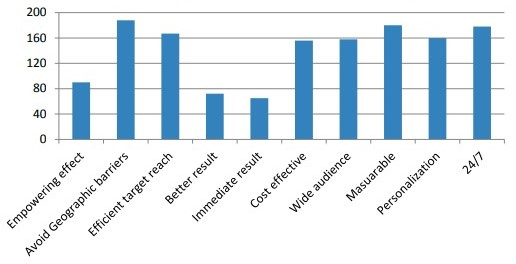
\includegraphics[width=7cm]{slika.prednosti.marketinga.jpg}
\end{center}
\caption{Prednosti internet marketinga}
\label{fig:prednosti}
\end{figure}
\end{frame}






\section{Razlike}
\begin{frame}{Razlike}
\begin{center}
\begin{tabular}{|p{2cm}|p{3.1cm}|p{3.1cm}|} \hline
     &\centering tradicionalan marketing& internet marketing\\ \hline
 \centering dopire do& ograničenog broja \centering ljudi & globalno\\   \hline
\centering pristupačnost & ograničena& široka i raznolika\\ \hline
\centering komunikacija & jednosmerna& dvosmerna\\\hline
 \centering vreme pristupanja& ograničeno& uvek dostupno \\ \hline
\centering ciljanje dobre  publike &  teško &  lako  \\ \hline
\end{tabular}
\label{tab:tabela1}
\end{center}
\end{frame}


\section{Mane Internet Marketinga}

\begin{frame}[fragile]\frametitle{Zašto je internet marketing loš?}
	\begin{itemize}	
		\item  Kopiranje
		\item  Nered na internetu
		\item  Neodgovarajući proizvodi
		\item  Konkurencija
		\item  Negativni komentari
		\item  Tehnologija je sklona kvaru
	\end{itemize}
\end{frame}



\section{Najvažniji elementi}

\begin{frame}[fragile]\frametitle{ Šta su najvažniji elementi?}
	\begin{itemize}	
		\item SEO optimizacija veb-sajta 
		\begin{itemize}
		    \item \large  ključne reči
		\end{itemize}
			\item Imejl marketing
			\begin{itemize}
			    \item Poziv na pretplatu na izveštaj
			    \item Promocije
			    \item Briga o kupcima
			    \item Imejl zahvalnica nakon kupovine
			\end{itemize}
			\item Plaćanje po kliku
			\item Marketing društvenih mreža
			\begin{itemize}
			    \item Različite promotivne aktivnosti
			    \item Influenseri
			\end{itemize}
			\item Povezivajuci marketing(eng.Afiliate marketing)
			\item Marketing preko pretraživačla(eng. Search Engine Marketing)
        		\item Kontent marketing
	\end{itemize}
\end{frame}

\begin{frame}[fragile]\frametitle{Zaključak}
	\begin{itemize}
		\item Konstantno razvijanje internet marketinga kao nove grane marketinga
        \item Rasteca popularnost internet marketinga medju raznim preduzetnicima
	\end{itemize}
\end{frame}
\end{document}



